\documentclass{article}
\setlength{\parskip}{0pt} % esp. entre parrafos
\setlength{\parindent}{20pt} % esp. al inicio de un parrafo
\usepackage{amsmath} % mates
\usepackage{listings}
\usepackage[sort&compress,numbers]{natbib} % referencias
\usepackage{url} % que las URLs se vean lindos
\usepackage[top=10mm,left=20mm,right=20mm,bottom=25mm]{geometry} % \textbf{\textbf{}}margenes
\usepackage{hyperref} % ligas de URLs
\usepackage{graphicx} % poner figuras
\usepackage[spanish]{babel} % otros idiomas
\hypersetup{
    colorlinks=true,
    linkcolor=blue,
    filecolor=blue,      
    urlcolor=blue,
}
\renewcommand{\lstlistingname}{C\'odigo}

\title{Reporte 2:\\Aut\'omata Celular}
\author{Jorge Torres}
\date{\today}

\begin{document}

\maketitle

\section{Objetivo}
El objetivo de la pr\'actica se centra en diseñar y ejecutar un experimento con por lo menos 30 r\'eplicas para estimar la probabilidad de creaci\'on de vida dentro de 200 iteraciones, usando niveles de 10, 15, 20 y 25 para el tamaño de matriz y los niveles 0.2, 0.4, 0.6 y 0.8 para la densidad inicial de vida.

\section{Desarrollo}
Utilizando como base el \href{https://github.com/satuelisa/Simulation/blob/master/CellularAutomata/gameOfLife.py}{c\'odigo} desarrollado por E. Schaeffer \cite{elisa1}, para generar un aut\'omata celular, primero se definen los tamaños de matriz, las densidades iniciales de vida, la cantidad de r\'eplicas y las iteraciones que dura el experimento. Estos par\'ametros se observan en el c\'odigo \ref{codigo1}. En seguida se definen dos funciones, \texttt{mapeo} y \texttt{paso}, que sirven respectivamente para: 1) mapear la matriz en cuesti\'on y 2) revisar la condici\'on de vida de cada celda individual en la matriz, la cual consiste en tener exactamente tres vecinos vivos (ver c\'odigo \ref{codigo2}). Por \'ultimo, se comienzan los ciclos \texttt{for} para iterar entre los par\'ametros definidos. En el ciclo donde se llama a la funci\'on \texttt{paso} se determina si el sistema termina en un estado de vida, para lo cual se lleva un contador que se usa posteriormente para determinar el porcentaje de supervivencia de acuerdo a la ecuaci\'on \ref{eq1},

\begin{equation}
    P_{s}=\frac{C_{v}}{R} \times 100
    \label{eq1}
\end{equation}
donde $P_{s}$ es el porcentaje de supervivencia, $C_{v}$ es la cantidad de sistemas que lograron sobrevivir y $R$ es la cantidad de veces que se replic\'o el experimento. Estas iteraciones se pueden apreciar en el c\'odigo \ref{codigo3}, mientras que el c\'odigo completo se puede revisar en mi \href{https://github.com/FeroxDeitas/Simulacion-Nano/blob/main/Tareas/P2/game_life.py}{repositorio} de GitHub.\\

\begin{lstlisting}[caption=Par\'ametros, label=codigo1, captionpos=b, language=Python]
dim = [10, 15, 20, 25] #matrix sizes
p = [0.2, 0.4, 0.6, 0.8] #initial life density
runs = 30 #replicas of the experiment
dur = 200 #iterations
\end{lstlisting}

\begin{lstlisting}[caption=Funciones, label=codigo2, captionpos=b, language=Python]
def mapeo(pos):
    fila = pos // lado
    columna = pos % lado
    return actual[fila, columna]

def paso(pos):
    fila = pos // lado
    columna = pos % lado
    vecindad = actual[max(0, fila - 1):min(lado, fila + 2),
                      max(0, columna - 1):min(lado, columna + 2)]
    return 1 * (np.sum(vecindad) - actual[fila, columna] == 3)

\end{lstlisting}

\newpage

\begin{lstlisting}[caption=Iteraci\'on de Par\'ametros, label=codigo3, captionpos=b, language=Python]
for lado in dim:
    num = lado**2
    for densidad in p:
        contador_viv=0
        for rep in range(runs):
            valores = [1 * (random() < densidad) for i in range(num)]
            actual = np.reshape(valores, (lado, lado))
            assert all([mapeo(x) == valores[x]  for x in range(num)])
            for iteracion in range(dur):
                valores = [paso(y) for y in range(num)]
                vivos = sum(valores)
                if vivos == 0:
                    break;
                if iteracion == (dur-1):
                    contador_viv += 1
                actual = np.reshape(valores, (lado, lado))
        vivieron = ((contador_viv*100)/(runs))
        resultados = {'Tamano matriz': lado,
                      'P inicial': densidad,
                      'Porcentaje Supervivencia(%)': vivieron}
        datos = datos.append(resultados, ignore_index=True)
\end{lstlisting}

\section{Resultados}
En la figura \ref{figura1} se observa el comportamiento del aut\'omata celular conforme se var\'ian el tamaño de matriz y la densidad inicial de vida.

\begin{figure}[h]
    \centering
    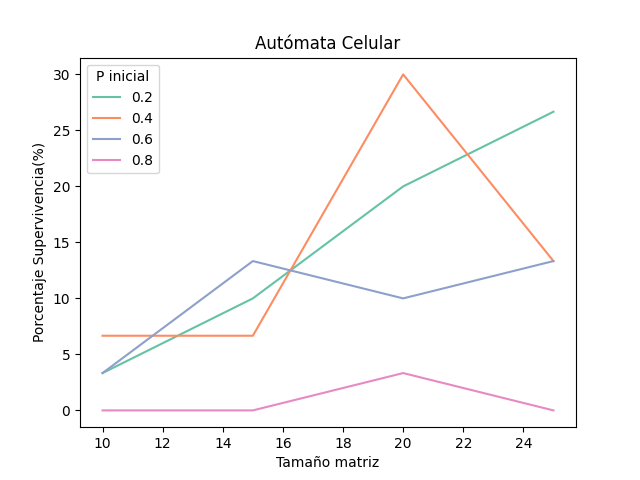
\includegraphics[width=140mm]{CellularAutomata.png}
    \caption{Porcentajes de supervivencia para sistemas con tamaños de matriz 10, 15, 20 y 25, y para densidades iniciales de vida de 0.2, 0.4, 0.6 y 0.8}
    \label{figura1}
\end{figure}

\section{Conclusiones}
Una observaci\'on inicial indica que los sistemas tienen una mayor probabilidad de sobrevivir conforme se aumenta el tamaño de la matriz y para densidades iniciales de vida medias y bajas (0.2, 0.4). Esto puede deberse a que las c\'elulas tendr\'ian un mayor espacio para proliferar en un \'area m\'as grande y a que no tendr\'ian tanta competencia al haber menos densidad.

Algo que destaca es la baja o nula probabilidad de supervivencia de los sistemas con una densidad inicial de 0.8, esto debido a la condici\'on de supervivencia de tener exactamente tres vecinos vivos. Podr\'ia cambiarse la condici\'on para estimular un mejor o peor crecimiento, pero eso est\'a fuera del rango de estudio de esta pr\'actica.

\bibliography{tarea2}
\bibliographystyle{plainnat}

\end{document}
